\documentclass[border=10pt]{standalone}
\usepackage{tikz}
\usepackage[T1]{fontenc}
\usepackage{lmodern}
\usetikzlibrary{shapes.geometric, arrows.meta, positioning, fit, backgrounds, calc}

\begin{document}

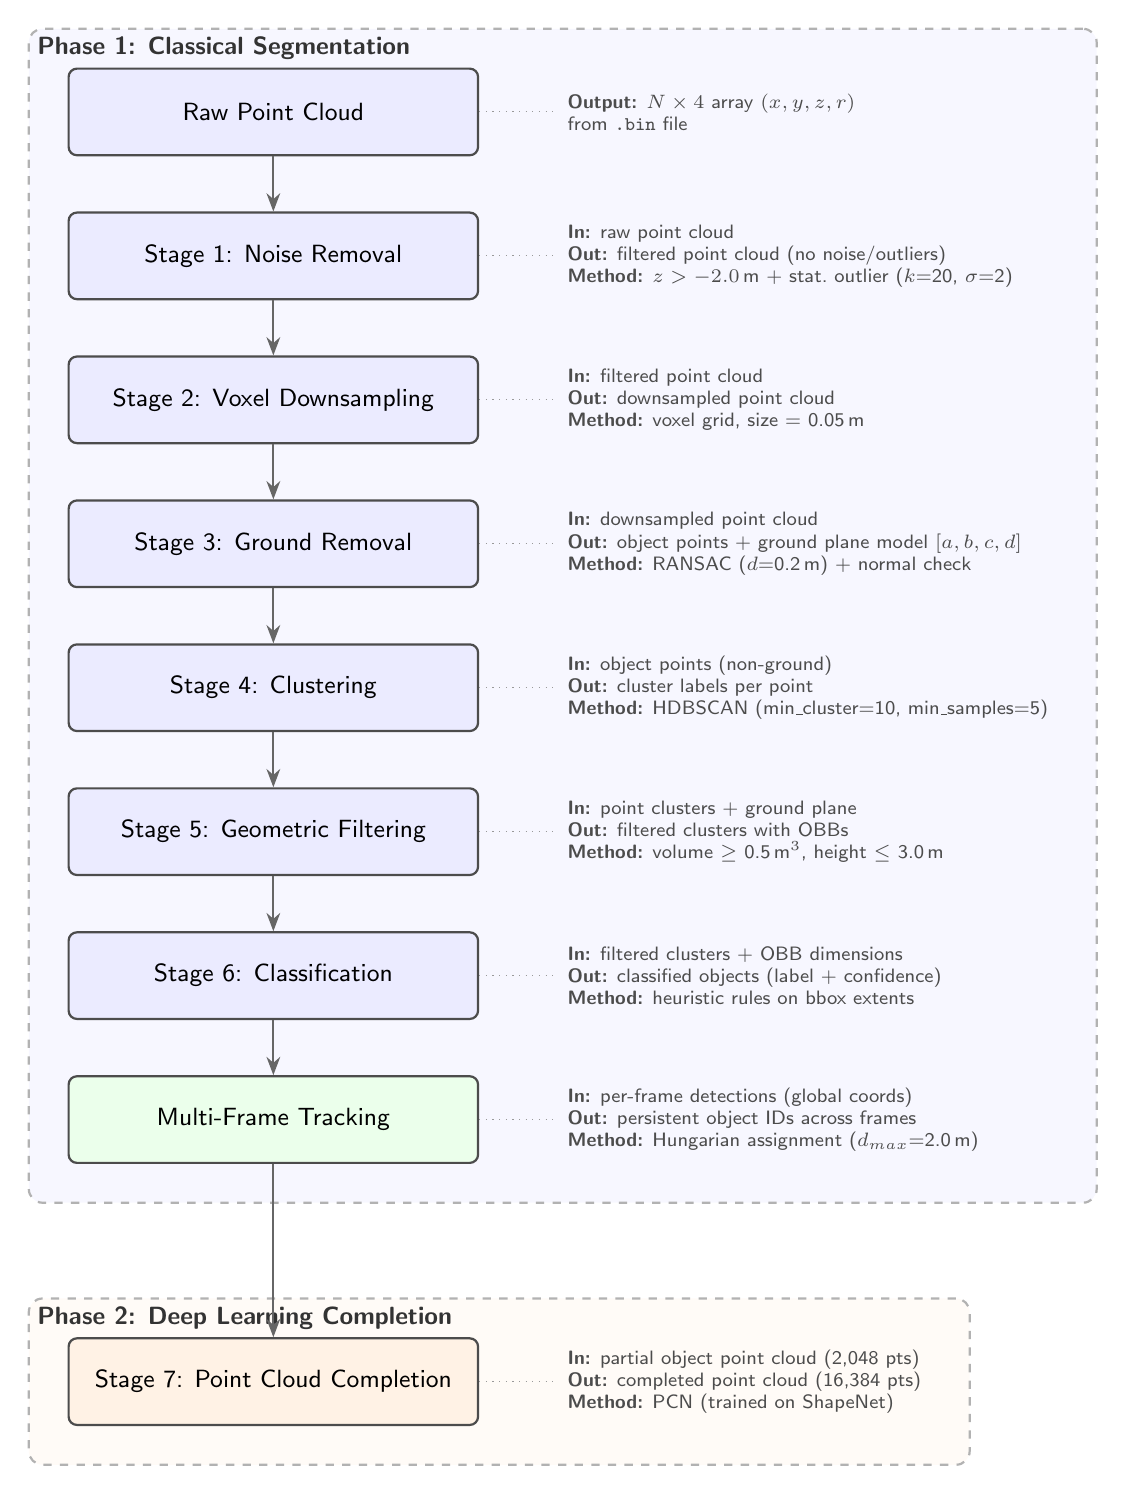
\begin{tikzpicture}[
    % Node styles
    stage/.style={
        rectangle, rounded corners=3pt, draw=black!70, thick,
        fill=blue!8, minimum width=5.2cm, minimum height=1.1cm,
        font=\sffamily\small, align=center, text=black
    },
    phase2stage/.style={
        rectangle, rounded corners=3pt, draw=black!70, thick,
        fill=orange!10, minimum width=5.2cm, minimum height=1.1cm,
        font=\sffamily\small, align=center, text=black
    },
    trackstage/.style={
        rectangle, rounded corners=3pt, draw=black!70, thick,
        fill=green!8, minimum width=5.2cm, minimum height=1.1cm,
        font=\sffamily\small, align=center, text=black
    },
    io/.style={
        font=\sffamily\scriptsize, text=black!70, align=left
    },
    arrow/.style={
        -Stealth, thick, black!60
    },
    phaselabel/.style={
        font=\sffamily\bfseries\small, text=black!80
    },
    phasebox/.style={
        rectangle, rounded corners=5pt, draw=black!30, dashed, thick,
        inner sep=12pt
    }
]

% --- Nodes ---
\node[stage] (input) {Raw Point Cloud};
\node[stage, below=0.7cm of input] (s1) {Stage 1: Noise Removal};
\node[stage, below=0.7cm of s1] (s2) {Stage 2: Voxel Downsampling};
\node[stage, below=0.7cm of s2] (s3) {Stage 3: Ground Removal};
\node[stage, below=0.7cm of s3] (s4) {Stage 4: Clustering};
\node[stage, below=0.7cm of s4] (s5) {Stage 5: Geometric Filtering};
\node[stage, below=0.7cm of s5] (s6) {Stage 6: Classification};
\node[trackstage, below=0.7cm of s6] (track) {Multi-Frame Tracking};
\node[phase2stage, below=2.2cm of track] (s7) {Stage 7: Point Cloud Completion};

% --- Arrows ---
\draw[arrow] (input) -- (s1);
\draw[arrow] (s1) -- (s2);
\draw[arrow] (s2) -- (s3);
\draw[arrow] (s3) -- (s4);
\draw[arrow] (s4) -- (s5);
\draw[arrow] (s5) -- (s6);
\draw[arrow] (s6) -- (track);
\draw[arrow] (track) -- (s7);

% --- Input/Output labels (right side) ---
% Input
\node[io, right=1.0cm of input] (io_input) {
    \textbf{Output:} $N \times 4$ array $(x, y, z, r)$\\
    from \texttt{.bin} file
};
\draw[dotted, black!40] (input.east) -- (io_input.west);

% Stage 1
\node[io, right=1.0cm of s1] (io_s1) {
    \textbf{In:} raw point cloud\\
    \textbf{Out:} filtered point cloud (no noise/outliers)\\
    \textbf{Method:} $z > -2.0$\,m + stat.\ outlier ($k$=20, $\sigma$=2)
};
\draw[dotted, black!40] (s1.east) -- (io_s1.west);

% Stage 2
\node[io, right=1.0cm of s2] (io_s2) {
    \textbf{In:} filtered point cloud\\
    \textbf{Out:} downsampled point cloud\\
    \textbf{Method:} voxel grid, size = 0.05\,m
};
\draw[dotted, black!40] (s2.east) -- (io_s2.west);

% Stage 3
\node[io, right=1.0cm of s3] (io_s3) {
    \textbf{In:} downsampled point cloud\\
    \textbf{Out:} object points + ground plane model $[a,b,c,d]$\\
    \textbf{Method:} RANSAC ($d$=0.2\,m) + normal check
};
\draw[dotted, black!40] (s3.east) -- (io_s3.west);

% Stage 4
\node[io, right=1.0cm of s4] (io_s4) {
    \textbf{In:} object points (non-ground)\\
    \textbf{Out:} cluster labels per point\\
    \textbf{Method:} HDBSCAN (min\_cluster=10, min\_samples=5)
};
\draw[dotted, black!40] (s4.east) -- (io_s4.west);

% Stage 5
\node[io, right=1.0cm of s5] (io_s5) {
    \textbf{In:} point clusters + ground plane\\
    \textbf{Out:} filtered clusters with OBBs\\
    \textbf{Method:} volume $\geq$ 0.5\,m$^3$, height $\leq$ 3.0\,m
};
\draw[dotted, black!40] (s5.east) -- (io_s5.west);

% Stage 6
\node[io, right=1.0cm of s6] (io_s6) {
    \textbf{In:} filtered clusters + OBB dimensions\\
    \textbf{Out:} classified objects (label + confidence)\\
    \textbf{Method:} heuristic rules on bbox extents
};
\draw[dotted, black!40] (s6.east) -- (io_s6.west);

% Tracking
\node[io, right=1.0cm of track] (io_track) {
    \textbf{In:} per-frame detections (global coords)\\
    \textbf{Out:} persistent object IDs across frames\\
    \textbf{Method:} Hungarian assignment ($d_{max}$=2.0\,m)
};
\draw[dotted, black!40] (track.east) -- (io_track.west);

% Stage 7
\node[io, right=1.0cm of s7] (io_s7) {
    \textbf{In:} partial object point cloud (2,048 pts)\\
    \textbf{Out:} completed point cloud (16,384 pts)\\
    \textbf{Method:} PCN (trained on ShapeNet)
};
\draw[dotted, black!40] (s7.east) -- (io_s7.west);

% --- Phase labels and boxes ---
\begin{scope}[on background layer]
    \node[phasebox, fill=blue!3, inner sep=14pt,
        fit=(input)(track)(io_input)(io_s1)(io_s2)(io_s3)(io_s4)(io_s5)(io_s6)(io_track),
        label={[phaselabel, anchor=north west]north west:Phase 1: Classical Segmentation}
    ] (phase1box) {};

    \node[phasebox, fill=orange!3, inner sep=14pt,
        fit=(s7)(io_s7),
        label={[phaselabel, anchor=north west]north west:Phase 2: Deep Learning Completion}
    ] (phase2box) {};
\end{scope}

\end{tikzpicture}

\end{document}
